% KYUSHU UNIVERSITY beamer template (adapted)
% MapReduce: Simplified Data Processing on Large Clusters
% Dean & Ghemawat, OSDI 2004 — Paper presentation
% Course: INF-419 Principles of Distributed Systems
% Technical University of Crete

\documentclass[11pt]{beamer}

\usepackage{graphicx}
\usepackage{listings}

\usepackage[
	backend=biber,
	style=verbose,
	sorting=ynt
]{biblatex}

% --- Packages ---
\usepackage{booktabs}
\usepackage{tikz}
\usetikzlibrary{positioning, arrows.meta, shapes, fit, backgrounds, calc}
\usepackage{amsmath}
\usepackage{amssymb}
\usepackage{caption}

\lstset{
    basicstyle=\tiny\ttfamily,
    aboveskip=0pt,
    belowskip=0pt,
    lineskip=0.2ex,
    breaklines=true
}

\date[May 2026]{May 2026}

\addbibresource{references.bib}

\usetheme{Madrid}

\author[Technical University of Crete]{Alexis Moumtzis \and Konstantinos Pisimisis \and Michail Mesanagrenos}

\title[MapReduce on Kubernetes --- INF-419]{MapReduce: Simplified Data Processing on Large Clusters}

\subtitle{Jeffrey Dean \& Sanjay Ghemawat, OSDI 2004}


\setbeamertemplate{navigation symbols}{}

% Optional: show slide numbers at bottom right
% \setbeamertemplate{footline}[frame number]

\titlegraphic{
    \includegraphics[width=3cm]
    {Technical-University-of-Crete-TUC-logo.png}
}

\usepackage{Kyushu}

\begin{document}

% ------------------------------------------------------------------
% Title
% ------------------------------------------------------------------
\begin{frame}
  \titlepage
\end{frame}

% ------------------------------------------------------------------
% Outline
% ------------------------------------------------------------------
\begin{frame}{Outline}
  \tableofcontents[hideallsubsections]
\end{frame}

% ==================================================================
% 1. INTRODUCTION / MOTIVATION  (1--2 min)
% ==================================================================
\section{Introduction \& Motivation}

\begin{frame}{The Problem at Google (early 2000s)}
\begin{itemize}
  \item Conceptually \alert{simple} computations over \alert{huge} datasets:
  \begin{itemize}
    \item Inverted indices for web search
    \item Graph structure of the Web
    \item Log summaries per host, most frequent queries\ldots
  \end{itemize}
  \item Input size: \alert{terabytes -- petabytes} of data.
  \item Must finish in reasonable time $\Rightarrow$ \alert{distribute across thousands of machines}.
\end{itemize}

\vspace{0.4em}
\begin{block}{The pain point}
Every new computation reinvents: parallelization, data distribution, fault tolerance,
load balancing\ldots \textbf{Complex code obscures simple logic.}
\end{block}
\end{frame}

\begin{frame}{The MapReduce Idea}
\begin{itemize}
  \item Inspired by \texttt{map} and \texttt{reduce} primitives of Lisp / functional languages.
  \item User writes only \alert{two pure functions}:
  \begin{itemize}
    \item \texttt{map(k1, v1)} $\rightarrow$ \texttt{list(k2, v2)}
    \item \texttt{reduce(k2, list(v2))} $\rightarrow$ \texttt{list(v2)}
  \end{itemize}
  \item The \alert{runtime} handles everything else:
        partitioning, scheduling, shuffling, failure recovery, straggler mitigation.
\end{itemize}

\begin{alertblock}{Why it matters}
Turns a distributed-systems problem into a \textbf{library call}.
Non-experts ran 1000-node jobs after a few days of training.
\end{alertblock}
\end{frame}

% ==================================================================
% 2. RELATED WORK  (2--3 min)
% ==================================================================
\section{Related Work}

\begin{frame}{Where MapReduce Stands}
\small
\begin{itemize}
  \item \alert{Bulk Synchronous Parallel (BSP)} \textit{[Valiant, 1990]}:
        global synchronization barriers; MapReduce uses a single barrier (shuffle).
  \item \alert{MPI / message passing}: expressive but \textbf{exposes} the network and failures to the user.
  \item \alert{Active Disks / River} \textit{[Acharya'98, Arpaci-Dusseau'99]}:
        push computation to data --- MapReduce inherits the data-locality principle.
  \item \alert{NOW-Sort / Charlotte / Condor}: cluster job schedulers, but no integrated
        programming model for data-parallel jobs.
\end{itemize}

\begin{block}{The contribution}
MapReduce \textbf{combines} a restricted programming model + an automatic runtime
+ commodity-hardware fault tolerance into a \textit{single} system used in production.
\end{block}
\end{frame}

\begin{frame}{Context inside Google}
\begin{itemize}
  \item \alert{GFS} (Google File System, SOSP 2003) --- the substrate:
        replicated, chunk-based, locality-aware DFS.
  \item \alert{Bigtable} (OSDI 2006) --- later built \textit{on top of} MapReduce and GFS.
  \item MapReduce became the de-facto interface to GFS for batch analytics.
\end{itemize}

\vspace{0.5em}
\begin{itemize}
  \item Open-source descendants:
        \alert{Apache Hadoop}, \alert{Apache Spark} (RDD/DAG generalization),
        \alert{Flink} (streaming), Google \alert{Dataflow}/\alert{Beam}.
\end{itemize}
\end{frame}

% ==================================================================
% 3. TECHNICAL PART  (8--9 min)
% ==================================================================
\section{Technical Part: KubeMapReduce}

\begin{frame}{From the 2004 Paper to a Cloud-Native System}
We re-implement the MapReduce paradigm on \alert{Kubernetes} with a different set
of building blocks --- the programming model stays, almost every runtime
decision changes.

\vspace{0.3em}
\scriptsize
\begin{table}
\centering
\begin{tabular}{lll}
\toprule
Concern              & Dean \& Ghemawat 2004     & \textbf{KubeMapReduce 2026} \\
\midrule
Master               & 1 process, checkpointed   & \alert{StatefulSet}, 3 replicas, FNV-1a sharded \\
Worker liveness      & Periodic ping             & \alert{gRPC heartbeats + leases} (TTL 30\,s) \\
Intermediate storage & Mapper local disk         & \alert{MinIO} object store + attempt-id paths \\
Data locality        & GFS chunk replicas        & \alert{K8s pod affinity} to MinIO topology zone \\
RPC                  & Custom                    & \alert{gRPC / Protobuf} over HTTP/2 \\
mTLS / policy        & ---                       & \alert{Linkerd} service mesh, per-method timeouts \\
Retry policy         & Library-driven            & \alert{Manager-driven}; \texttt{backoffLimit:\,0} \\
Code execution       & Single C++ binary         & Any \alert{Python / Java / C/C++} via stdio \\
External access      & Internal cluster          & \alert{Gateway API} + TLS at the edge \\
\bottomrule
\end{tabular}
\end{table}
\end{frame}

\begin{frame}{Three-Layer Microservice Architecture}
\centering
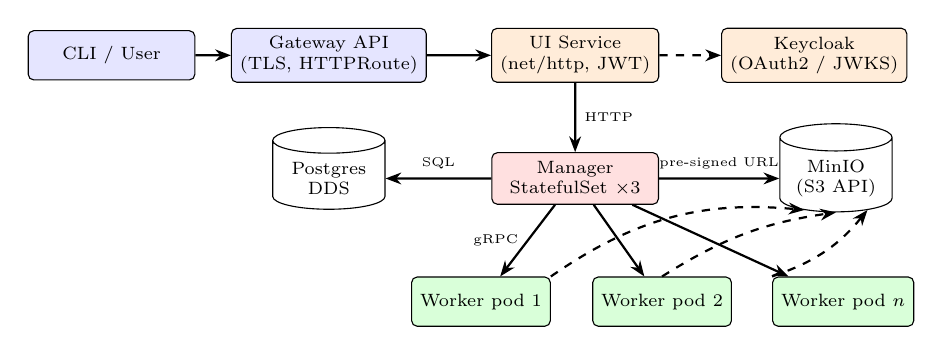
\begin{tikzpicture}[
            scale=0.92,
            transform shape,
            every node/.style={font=\scriptsize},
            box/.style={draw, rounded corners=2pt, minimum width=2.3cm, minimum height=0.68cm, align=center},
            db/.style={draw, cylinder, shape border rotate=90, aspect=0.28,
                                           minimum height=0.92cm, minimum width=1.55cm, align=center},
            arrow/.style={-{Stealth[length=2mm]}, thick}
      ]
      % Top row
      \node[box, fill=blue!10] (cli) at (-4.8, 2.2) {CLI / User};
      \node[box, fill=blue!10] (gw)  at (-1.8, 2.2) {Gateway API\\(TLS, HTTPRoute)};
      \node[box, fill=orange!15] (ui) at (1.6, 2.2) {UI Service\\(net/http, JWT)};
      \node[box, fill=orange!15] (kc) at (4.9, 2.2) {Keycloak\\(OAuth2 / JWKS)};

      % Core row
      \node[db] (pg) at (-1.8, 0.5) {Postgres\\DDS};
      \node[box, fill=red!12] (mgr) at (1.6, 0.5) {Manager\\StatefulSet $\times 3$};
      \node[db] (s3) at (5.2, 0.5) {MinIO\\(S3 API)};

      % Worker row
      % Worker row
\node[
    box,
    fill=green!15,
    minimum width=1.7cm   % smaller width
] (w1) at (0.3, -1.2) {Worker pod 1};

\node[
    box,
    fill=green!15,
    minimum width=1.7cm
] (w2) at (2.8, -1.2) {Worker pod 2};

\node[
    box,
    fill=green!15,
    minimum width=1.7cm
] (wn) at (5.3, -1.2) {Worker pod $n$};

      \draw[arrow] (cli) -- (gw);
      \draw[arrow] (gw) -- (ui);
      \draw[arrow, dashed] (ui) -- (kc);

      \draw[arrow] (ui) -- node[midway, right, font=\tiny]{HTTP} (mgr);
      \draw[arrow] (mgr) -- node[midway, above, font=\tiny]{SQL} (pg);
      \draw[arrow] (mgr) -- node[midway, above, font=\tiny]{pre-signed URL} (s3);

      \draw[arrow] (mgr) -- node[midway, left, font=\tiny]{gRPC} (w1);
      \draw[arrow] (mgr) -- (w2);
      \draw[arrow] (mgr) -- (wn);

      \draw[arrow, dashed] (w1.north east) to[bend left=20] (s3.south west);
      \draw[arrow, dashed] (w2.north) to[bend left=12] (s3.south);
      \draw[arrow, dashed] (wn.north west) to[bend right=16] (s3.south east);
\end{tikzpicture}

\vspace{0.4em}
\scriptsize
\textbf{Trust boundary}: CLI / UI handle JWTs; the Manager and Workers \alert{never see user tokens} ---
they use Kubernetes Secrets and per-task pre-signed URLs.
\end{frame}

\begin{frame}[fragile]{Programming Model (unchanged from the paper)}
\begin{block}{User supplies two stdio programs}
\begin{lstlisting}
mapper.{py,jar,c,cpp}:  reads JSONL from stdin  -> writes JSONL to stdout
reducer.{py,jar,c,cpp}: reads JSONL from stdin  -> writes JSONL to stdout
\end{lstlisting}
\end{block}

\textbf{WordCount mapper (Python, from \texttt{benchmarks/wordcount/}):}
\begin{lstlisting}[language=Python]
import sys, json, re
for line in sys.stdin:
    rec = json.loads(line)
    for w in re.findall(r"[a-z']+", rec["value"].lower()):
        print(json.dumps({"key": w, "value": "1"}))
\end{lstlisting}

\scriptsize
The Go Worker \alert{spawns the user binary as a child process}
(\texttt{os/exec}) with a sandboxed env (allowlist: \texttt{PATH, HOME, USER, LANG,
TMPDIR, TZ, TASK\_ID, JOB\_ID}) --- \textbf{no MinIO or DB credentials are exposed}.
\end{frame}

\begin{frame}[fragile]{Manager Sharding: FNV-1a on \texttt{job\_id}}
3 Manager replicas (\texttt{manager-0..2.manager-headless}) share one Postgres DDS.
A new job is \alert{deterministically routed} to a single replica:

\vspace{0.8em}
\begin{lstlisting}
replica(job_id) = FNV-1a(job_id) mod N      // N = STATEFULSET_REPLICAS = 3
addr           = "manager-{i}.manager-headless.mapreduce.svc.cluster.local"
\end{lstlisting}

\begin{itemize}\small
  \item ``Each job has exactly one master''  $\Rightarrow$ satisfied by the hash, not by a leader election.
  \item Manager state is \alert{stateless in-process}: every transition is persisted to Postgres.
  \item On crash, K8s respawns \texttt{manager-i} with the same DNS name;
        it re-reads \texttt{replica\_index} from \texttt{TASKS} and resumes orchestration.
  \item DDS still uses \alert{\texttt{SELECT ... FOR UPDATE SKIP LOCKED}} on task assignment
        so two replicas can never schedule the same task during a rebalance.
\end{itemize}
\end{frame}

% ------------------------------------------------------------------
% NEW: Distributed Data Store schema
% ------------------------------------------------------------------
\begin{frame}[fragile]{The Distributed Data Store (Postgres)}
A single source of truth for 3 stateless Managers --- \alert{every state transition is a SQL transaction}.

\vspace{0.4em}
\scriptsize
\begin{table}
\centering
\begin{tabular}{lll}
\toprule
Table             & Key columns                                              & Role \\
\midrule
\texttt{JOBS}             & \texttt{job\_id}, \texttt{status}, \texttt{user\_id}                        & lifecycle FSM \\
\texttt{JOB\_CONFIGS}     & \texttt{mapper\_uri}, \texttt{m\_tasks}, \texttt{r\_tasks}                  & immutable spec \\
\texttt{TASKS}            & \texttt{task\_id}, \texttt{status}, \alert{\texttt{current\_attempt\_id}}   & fencing pointer \\
\texttt{TASK\_INPUTS}     & \texttt{byte\_start/\_end}, \texttt{split\_checksum}                        & 1NF splits \\
\texttt{TASK\_ATTEMPTS}   & \texttt{attempt\_id}, \texttt{lease\_id}, \texttt{last\_renewed\_at}        & liveness + identity \\
\texttt{TASK\_OUTPUTS}    & \texttt{output\_uri}, \texttt{checksum}                                     & 1NF results (no JSON blobs) \\
\texttt{SYSTEM\_CONFIG}   & \texttt{max\_concurrent\_pods}, locality keys                               & admin-tunable knobs \\
\bottomrule
\end{tabular}
\end{table}

\vspace{0.3em}
\begin{lstlisting}[language=SQL]
-- Scheduler dequeue: 3 managers, zero double-scheduling
SELECT task_id FROM tasks
 WHERE status = 'Idle' AND replica_index = $1
 ORDER BY created_at
 FOR UPDATE SKIP LOCKED
 LIMIT $2;
\end{lstlisting}

\scriptsize
\textbf{Deliberate denormalization}: \texttt{TASKS.current\_attempt\_id} duplicates a row in
\texttt{TASK\_ATTEMPTS} so the commit check is \alert{one indexed lookup} ---
updated atomically with the attempt row in the same transaction.
\end{frame}

% ------------------------------------------------------------------
% NEW: Job / Task lifecycle FSM
% ------------------------------------------------------------------
\begin{frame}{Job \& Task Lifecycle (with the \texttt{Cleaning} Phase)}
\centering
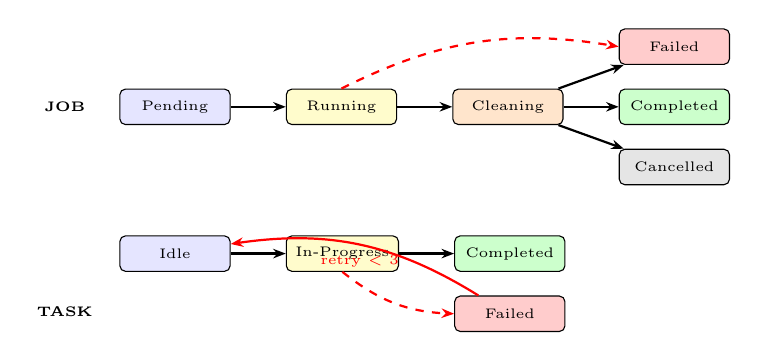
\begin{tikzpicture}[
    node distance=0.4cm and 0.7cm, every node/.style={font=\tiny},
    s/.style={draw, rounded corners=2pt, minimum width=1.4cm, minimum height=0.45cm, align=center},
    arrow/.style={-{Stealth[length=1.6mm]}, thick}
  ]
  % Job FSM (top)
  \node[s, fill=blue!10]   (jp) {Pending};
  \node[s, fill=yellow!20, right=of jp] (jr) {Running};
  \node[s, fill=orange!20, right=of jr] (jc) {Cleaning};
  \node[s, fill=green!20,  right=of jc] (jd) {Completed};
  \node[s, fill=red!20, above=0.3cm of jd] (jf) {Failed};
  \node[s, fill=gray!20, below=0.3cm of jd] (jx) {Cancelled};
  \draw[arrow] (jp) -- (jr);
  \draw[arrow] (jr) -- (jc);
  \draw[arrow] (jc) -- (jd);
  \draw[arrow] (jc) -- (jf);
  \draw[arrow] (jc) -- (jx);
  \draw[arrow, red, dashed] (jr.north) to[bend left=18] (jf.west);
  \node[font=\tiny] at (-1.4, 0) {\textbf{JOB}};

  % Task FSM (bottom)
  \node[s, fill=blue!10, below=1.4cm of jp]   (ti) {Idle};
  \node[s, fill=yellow!20, right=of ti] (tp) {In-Progress};
  \node[s, fill=green!20, right=of tp]  (tc) {Completed};
  \node[s, fill=red!20, below=0.3cm of tc]   (tf) {Failed};
  \draw[arrow] (ti) -- (tp);
  \draw[arrow] (tp) -- (tc);
  \draw[arrow, red, dashed] (tp.south) to[bend right=18] (tf.west);
  \draw[arrow, red] (tf) to[bend right=20] node[below, font=\tiny]{retry $<$ 3} (ti);
  \node[font=\tiny] at (-1.4, -2.6) {\textbf{TASK}};
\end{tikzpicture}

\vspace{0.4em}
\scriptsize
\begin{itemize}
  \item \alert{\texttt{Cleaning} is mandatory}: before \textit{any} terminal state, the Manager
        bulk-deletes \texttt{staging/<job\_id>/} and removes \texttt{TASK\_ATTEMPTS} rows
        --- guarantees no orphan intermediate data.
  \item Task failure with \texttt{attempt\_count $<$ MaxTaskAttempts (3)} re-spawns an attempt;
        otherwise the parent JOB transitions to \texttt{Cleaning $\to$ Failed}.
  \item Orphan \texttt{temp/} uploads (presigned PUT never finalized) are reaped by
        a \alert{24\,h MinIO lifecycle policy} configured at service startup
        (\texttt{ensureTempLifecyclePolicy} in both API and Manager binaries,
        and the \texttt{minio-setup} Kubernetes Job), not by the Manager.
\end{itemize}
\end{frame}

\begin{frame}[fragile]{Lease-Based Fencing \& Attempt-ID Commits}
\textbf{Two interlocking mechanisms} in the \texttt{TASK\_ATTEMPTS} table:

\vspace{0.7em}
\begin{lstlisting}
attempt_id      UUID PK   -- new on every retry
lease_id        UUID      -- renewed on every Heartbeat
last_renewed_at TIMESTAMP -- expiry = last_renewed_at + lease_ttl
lease_ttl       INT       -- default 30 s, clock skew 5 s
\end{lstlisting}
\vspace{0.5em}

\textbf{Defaults in \texttt{manager-service/internal/manager/scheduler.go}}
\begin{itemize}\small
  \item \texttt{MaxTaskAttempts = 3} (then job is failed)
  \item \texttt{DefaultMaxConcurrentPods = 10} (quota in \texttt{SYSTEM\_CONFIG})
  \item \texttt{leaseClockSkewSeconds = 5} (tolerated drift)
\end{itemize}

\begin{alertblock}{Why two IDs?}
\texttt{lease\_id} fences the \alert{live} worker (TTL expiry).
\texttt{attempt\_id} fences the \alert{output}: Manager compares the inbound
\texttt{TaskComplete.attempt\_id} against \texttt{TASKS.current\_attempt\_id}
inside one SQL transaction --- stale zombies are silently rejected.
\end{alertblock}
\end{frame}

% ------------------------------------------------------------------
% NEW: Commit protocol pseudo-code
% ------------------------------------------------------------------
\begin{frame}[fragile]{The Commit Protocol in One Transaction}
Every \texttt{TaskComplete} RPC is validated by the \alert{same atomic SQL block} ---
this is what makes zombie writers harmless.

\vspace{0.3em}
\begin{lstlisting}[language=SQL]
BEGIN;

-- (1) Fence the live worker: lease must still be valid
UPDATE task_attempts
   SET status = 'Success', end_time = now()
 WHERE attempt_id = :inbound_attempt_id
   AND lease_id   = :inbound_lease_id
   AND last_renewed_at + (lease_ttl || ' seconds')::interval
       > now() - interval '5 seconds';      -- clockSkew
-- 0 rows updated  =>  ABORT, return Ack{accepted=false}

-- (2) Fence the output: must be the *current* attempt
UPDATE tasks
   SET status = 'Completed'
 WHERE task_id            = :inbound_task_id
   AND current_attempt_id = :inbound_attempt_id;
-- 0 rows updated  =>  stale attempt, ABORT (silently drop output)

-- (3) Persist 1NF output rows (one per partition)
INSERT INTO task_outputs(task_id, partition_index, output_uri, checksum)
VALUES (...);

COMMIT;                  -- only now is the result *committed*
\end{lstlisting}

\vspace{0.2em}
\scriptsize
Worker upload path is \alert{attempt-scoped}:
\texttt{staging/<job\_id>/<task\_id>/<attempt\_id>/part-<p>.jsonl}.
A zombie that wakes up after step (2) has already moved \texttt{current\_attempt\_id}
just writes into a directory \alert{nobody will ever read} --- and the bulk
\texttt{staging/<job\_id>/} delete in the \texttt{Cleaning} phase removes it.
\end{frame}

\begin{frame}{Heartbeats, the Active Reaper, and the Manager Loop}
\centering
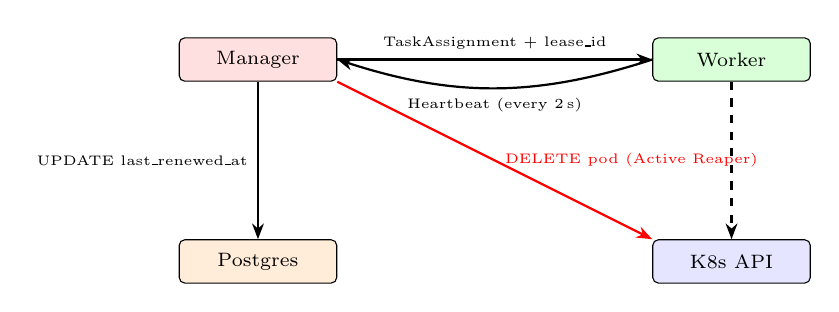
\begin{tikzpicture}[
    node distance=0.5cm and 0.7cm, every node/.style={font=\scriptsize},
    box/.style={draw, rounded corners=2pt, minimum width=2.0cm, minimum height=0.55cm, align=center},   
    arrow/.style={-{Stealth[length=2mm]}, thick}
  ]
\node[box, fill=red!12, xshift=-1.2cm]             (mgr) {Manager};

\node[box, fill=green!15,
      right=4cm of mgr]                          (w)   {Worker};

\node[box, fill=blue!10,
      below=2.0cm of w]                            (k8s) {K8s API};

\node[box, fill=orange!15,
      below=2.0cm of mgr]                          (db)  {Postgres};

  \draw[arrow] (mgr.east) -- node[above, font=\tiny]{TaskAssignment + lease\_id} (w.west);
  \draw[arrow] (w.west) to[bend left=18]
       node[below, font=\tiny]{Heartbeat (every 2\,s)} (mgr.east);
  \draw[arrow, dashed] (w) -- (k8s);
  \draw[arrow] (mgr) -- node[left, font=\tiny]{UPDATE last\_renewed\_at} (db);
  \draw[arrow, red, thick] (mgr.south east) -- node[right, font=\tiny]{DELETE pod (Active Reaper)} (k8s.north west);
\end{tikzpicture}

\vspace{0.3em}
\scriptsize
\begin{itemize}
  \item Heartbeat cadence: \texttt{HEARTBEAT\_INTERVAL\_SEC = 2}, \texttt{MAX\_MISSED\_HEARTBEATS = 5}.
  \item On missed heartbeats the Manager (i) marks the attempt \texttt{Failed},
        (ii) issues \texttt{DELETE} on the K8s Job + Pod, (iii) spawns a fresh
        attempt --- \textbf{Kubernetes never retries on its own} (\texttt{backoffLimit: 0},
        \texttt{restartPolicy: Never}).
  \item Cleanup pool: 4 reconciliation workers, batch size 64, up to 10 retries
        of \texttt{staging/<job\_id>/} delete before forcing terminal state.
\end{itemize}
\end{frame}

\begin{frame}[fragile]{The gRPC Contract (\texttt{proto/mapreduce.proto})}
\begin{lstlisting}
service WorkerService {
  rpc Register     (RegisterRequest)     returns (TaskAssignment);
  rpc Heartbeat    (HeartbeatRequest)    returns (HeartbeatResponse);
  rpc TaskComplete (TaskCompleteRequest) returns (Ack);
  rpc TaskFailed   (TaskFailedRequest)   returns (Ack);
  rpc TaskStream   (stream StreamRequest)
                                returns (stream StreamResponse);
}
service ShuffleService {
  rpc PushShuffleData (stream ShuffleDataChunk) returns (Ack);
  rpc GetShuffleData  (ShuffleDataRequest) returns (stream ShuffleDataChunk);
}
\end{lstlisting}

\scriptsize
\begin{itemize}
  \item Every RPC carries \texttt{task\_id, attempt\_id, lease\_id} for fencing.
  \item Auth via the \texttt{x-worker-token} gRPC metadata header (Manager-side interceptor;
        \texttt{codes.Unauthenticated} otherwise).
  \item \texttt{TaskStream} is a bi-directional stream for long-lived workers ---
        registration, heartbeats and completions multiplexed on \alert{one HTTP/2 connection}.
  \item \alert{Manifest fallback}: if \texttt{data\_locations} for a Reducer would exceed
        the 4\,MB gRPC frame, Manager uploads a JSON manifest to MinIO and sets
        \texttt{is\_manifest = true}.
\end{itemize}
\end{frame}

\begin{frame}{Linkerd Service Mesh: mTLS + Per-Method Policy}
We don't trust the cluster network. \alert{Linkerd 2.15+} sidecars give us automatic
mTLS (\textbf{24\,h cert rotation}) and \textit{per-RPC-method} traffic policy.

\vspace{0.3em}
\begin{table}
\centering
\scriptsize
\begin{tabular}{lccl}
\toprule
RPC / target              & Timeout & Retries & Rationale \\
\midrule
\texttt{Heartbeat}        & 2\,s   & \alert{0} & Must fail-fast $\to$ Reaper signal \\
\texttt{Register}         & 5\,s   & 3 (exp.\ backoff) & Task startup overhead \\
\texttt{TaskComplete}     & 10\,s  & 2 (exp.\ backoff) & Atomic commit, idempotent on attempt-id \\
\texttt{TaskFailed}       & 10\,s  & 2                & Same as above \\
Manager $\to$ PostgreSQL  & 30\,s  & \alert{0}        & Non-idempotent, circuit-break $>$50\% errors \\
Manager $\to$ MinIO       & 60\,s  & 3                & Large object I/O, idempotent \\
\bottomrule
\end{tabular}
\end{table}

\vspace{0.3em}
\scriptsize
\textbf{Defence in depth} (\texttt{docs/TIMEOUT\_CONFIGURATION.md}): Go gRPC
interceptors enforce the same budgets in-process, so a Linkerd outage
\alert{does not} expose us to hung connections.
\end{frame}

\begin{frame}[fragile]{Worker Pipeline: from Split to Partitioned Output}
\centering
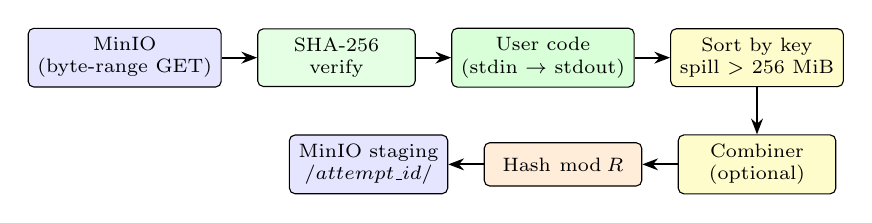
\begin{tikzpicture}[
    node distance=0.4cm and 0.45cm, every node/.style={font=\scriptsize},
    box/.style={draw, rounded corners=2pt, minimum width=2.0cm, minimum height=0.55cm, align=center},
    arrow/.style={-{Stealth[length=2mm]}, thick}
  ]
  \node[box, fill=blue!10]                  (s3a) {MinIO\\(byte-range GET)};
  \node[box, fill=green!10, right=of s3a]   (chk) {SHA-256\\verify};
  \node[box, fill=green!15, right=of chk]   (usr) {User code\\(stdin $\to$ stdout)};
  \node[box, fill=yellow!20, right=of usr]  (srt) {Sort by key\\spill $>$ 256 MiB};
  \node[box, fill=yellow!20, below=0.6cm of srt] (cmb) {Combiner\\(optional)};
  \node[box, fill=orange!15, left=of cmb]   (par) {Hash $\bmod\,R$};
  \node[box, fill=blue!10, left=of par]     (s3b) {MinIO staging\\/$attempt\_id$/};

  \draw[arrow] (s3a) -- (chk);
  \draw[arrow] (chk) -- (usr);
  \draw[arrow] (usr) -- (srt);
  \draw[arrow] (srt) -- (cmb);
  \draw[arrow] (cmb) -- (par);
  \draw[arrow] (par) -- (s3b);
\end{tikzpicture}

\vspace{0.3em}
\scriptsize
\textbf{Concrete defaults} (\texttt{worker-service/internal/config}):
\texttt{MAP\_SORT\_SPILL\_THRESHOLD\_MB = 256},
\texttt{SHUFFLE\_BATCH\_SIZE = 500} (hard cap \texttt{MaxBatchSize = 900} to stay under the
1024 fd ulimit), \texttt{SHUFFLE\_MAX\_RECORD\_BYTES = 1 MiB},
shuffle chunk size 1\,MiB. Output written directly into
\texttt{staging/<job\_id>/<task\_id>/<attempt\_id>/part-<p>.jsonl}.
\end{frame}

\begin{frame}{Record-Boundary \& Checksum Discipline}
\begin{columns}[T]
\column{0.5\textwidth}
\textbf{JSONL byte-range splits}
\begin{itemize}\scriptsize
  \item If \texttt{byte\_start $>$ 0}: peek byte at \texttt{byte\_start-1}.
        Not a \texttt{\textbackslash n}? Discard up to the next newline ---
        previous worker owns this record.
  \item Always read \alert{past} \texttt{byte\_end} until the next newline ---
        \textbf{never truncate the tail record}.
\end{itemize}

\column{0.5\textwidth}
\textbf{End-to-end SHA-256}
\begin{itemize}\scriptsize
  \item \alert{Map-read}: hash bytes after the range fetch,
        compare to \texttt{TASK\_INPUTS.split\_checksum}; mismatch $\to$ fail attempt.
  \item \alert{Shuffle-merge}: Reducer re-hashes each partition file
        against \texttt{TASK\_OUTPUTS.checksum} before merging.
  \item Closes the door on \textbf{silent corruption} from MinIO erasure-decode bugs
        or torn writes.
\end{itemize}
\end{columns}

\vspace{0.5em}
\begin{block}{Multi-pass external merge sort (\texttt{shuffle/merge.go})}
Min-heap over a batch of $\le 500$ streams $\to$ spill files $\to$ final pass.
Memory bounded by $O(\text{batch\_size})$, \textbf{not} $O(M)$.
\end{block}
\end{frame}

\begin{frame}{Data-Locality-Aware Scheduling (beyond the design doc)}
The paper exploits \textbf{GFS chunk locality}; we don't have GFS, but we still
want compute close to MinIO.

\vspace{0.3em}
\textbf{Mechanism} (\texttt{migrations/0002\_add\_locality\_config.sql} +
\texttt{ARCHITECTURE\_DATA\_LOCALITY.md})
\begin{itemize}\small
  \item Manager injects a K8s \alert{soft pod affinity}
        (\texttt{preferredDuringSchedulingIgnoredDuringExecution}, weight 100)
        into every worker Job manifest.
  \item Defaults: \texttt{locality\_key = topology.kubernetes.io/zone},
        \texttt{label\_selector = app.kubernetes.io/name=minio}.
  \item Admin-tunable per cluster:
        \texttt{kubemapreduce admin configure-nodes --locality-key kubernetes.io/hostname}
        for same-node affinity, or empty string to disable.
\end{itemize}

\begin{alertblock}{Honest about the limit}
This is \alert{storage-tier locality}, \textbf{not per-split data locality}.
All workers of a job share the same affinity rule --- we steer the pool toward the
MinIO zone but we do not (yet) place each Map task on the node that holds its bytes.
\end{alertblock}
\end{frame}

\begin{frame}{Storage \& Trust: Pre-Signed URLs + Gateway API}
\begin{columns}[T]
\column{0.55\textwidth}
\textbf{Zero-trust object access}
\begin{itemize}\scriptsize
  \item User uploads/downloads only via short-lived
        \alert{S3 pre-signed PUT/GET URLs} issued by the UI.
  \item Orphan mitigation: uploads land under \texttt{temp/}, swept by a MinIO
        \alert{24\,h lifecycle policy}; final job commit copies to \texttt{inputs/}
        server-side.
  \item Workers receive MinIO credentials only via K8s Secret refs
        (\texttt{secretKeyRef: minio-creds}); never inlined.
\end{itemize}

\column{0.45\textwidth}
\textbf{External routing}
\begin{itemize}\scriptsize
  \item Kubernetes \alert{Gateway API} (\texttt{k8s/60-gateway.yaml})
        $\to$ 3 HTTPRoutes:
        \begin{itemize}\tiny
          \item \texttt{api.mapreduce.local} $\to$ UI
          \item \texttt{storage.mapreduce.local} $\to$ MinIO
          \item \texttt{auth.mapreduce.local} $\to$ Keycloak
        \end{itemize}
  \item \alert{TLS termination at the Gateway} (port 443),
        port 80 returns \texttt{HTTP 301} to HTTPS.
\end{itemize}
\end{columns}

\vspace{0.4em}
\scriptsize
\textbf{Authentication}: CLI runs the OAuth2 Password Grant against Keycloak,
caches tokens under \texttt{\textasciitilde/.mapreduce/config.json} with \texttt{chmod 600},
proactively refreshes within a 30-second skew window. The UI Service is
\alert{stateless} --- it only validates the bearer JWT (via JWKS) per request.
\end{frame}

% ==================================================================
% 4. EXPERIMENTS  (2--3 min)
% ==================================================================
\section{Experiments}

\begin{frame}{Benchmark Suite (\texttt{benchmarks/})}
Two reference workloads ship with the repo, driven by a real-world corpus.

\vspace{0.3em}
\textbf{Corpus} (\texttt{benchmarks/build\_corpus.py})
\begin{itemize}\small
  \item 6 Project Gutenberg books $\to$ stripped to JSONL.
  \item \texttt{corpus.jsonl}: $\approx$\alert{77\,517 lines}, one record per text line:
        \texttt{\{"key": "pg1342:000042", "value": "It is a truth..."\}}.
\end{itemize}

\vspace{0.4em}
\begin{table}
\centering
\scriptsize
\begin{tabular}{lll}
\toprule
Benchmark             & Mapper                              & Reducer / output \\
\midrule
\alert{WordCount}     & Tokenize line, emit $(w, 1)$        & Sum counts per word \\
\alert{Distributed Grep} & Emit record if \texttt{re.search(GREP\_PATTERN, value)}
                                                            & Identity \\
\bottomrule
\end{tabular}
\end{table}

\vspace{0.4em}
Each suite ships a \texttt{validate.py} that runs the pipeline \textbf{locally}
and a \texttt{--compare} mode that diffs the cluster output against the local
oracle --- our \alert{correctness gate} in CI.
\end{frame}

\begin{frame}{Test Cluster \& What We Measure}
\textbf{Setup}
\begin{itemize}\small
  \item Target: \alert{8-node Okeanos cluster} (project requirement).
  \item Local dev: \texttt{minikube} via \texttt{scripts/} +
        \texttt{k8s/kustomization.yaml}.
  \item Manager: StatefulSet, 3 replicas. Default quota: 10 concurrent worker pods.
\end{itemize}

\vspace{0.3em}
\textbf{Built-in Prometheus metrics} (\texttt{/metrics} on Manager)
\begin{table}
\centering
\scriptsize
\begin{tabular}{ll}
\toprule
Metric                                            & What it tells us \\
\midrule
\texttt{kubemapreduce\_tasks\_scheduled\_total}   & throughput (split by Map/Reduce) \\
\texttt{kubemapreduce\_tasks\_completed\_total}   & success counter \\
\texttt{kubemapreduce\_tasks\_failed\_total}      & failures \\
\texttt{kubemapreduce\_heartbeats\_total}         & liveness, split CONTINUE/TERMINATE \\
\texttt{kubemapreduce\_reaper\_recovered\_total}  & \alert{Active Reaper effectiveness} \\
\texttt{kubemapreduce\_reaper\_cycle\_seconds}    & reaper loop latency (histogram) \\
\texttt{kubemapreduce\_http\_request\_duration\_seconds} & API SLI \\
\bottomrule
\end{tabular}
\end{table}

\scriptsize
\textbf{Success rate} $= \mathrm{completed} / (\mathrm{completed} + \mathrm{failed})$.\quad
\textbf{Auto-recovery} $= \mathrm{reaper\_recovered} / \mathrm{failed}$.
\end{frame}

\begin{frame}{Chaos \& Failure Injection (\texttt{e2e/}, \texttt{k8s/chaos/})}
We don't just \emph{describe} fault tolerance --- we \alert{inject the faults} in CI.

\vspace{0.3em}
\textbf{Scenarios exercised by \texttt{e2e/chaos\_test.go} and \texttt{e2e/failure\_injection\_test.go}}
\begin{itemize}\small
  \item \alert{Worker preemption}: \texttt{kubectl delete pod} on an in-progress worker.
        Expectation: Reaper detects 5 missed heartbeats, deletes the K8s Job,
        re-schedules; job still completes.
  \item \alert{Manager preemption}: kill the replica that owns the job.
        Expectation: K8s respawns \texttt{manager-i}, new pod resumes
        orchestration from Postgres state.
  \item \alert{Network delay} (\texttt{k8s/chaos/01-manager-network-delay.yaml}):
        inject latency on the Manager $\to$ Worker path. Expectation: gRPC
        timeouts trigger, no stuck tasks.
  \item \alert{Keycloak partition} (\texttt{02-keycloak-partition.yaml}):
        identity provider unreachable. Expectation: \textit{already-submitted} jobs
        keep running; new logins fail with a clear 401.
\end{itemize}

\begin{block}{What we validate}
The job \alert{completes} and the output \alert{matches the local oracle}
(byte-for-byte after sorting) --- even when each scenario is injected.
\end{block}
\end{frame}

\begin{frame}{API Load Testing (\texttt{scripts/load\_test.js})}
\textbf{Tooling}
\begin{itemize}\small
  \item \texttt{k6} script driving \texttt{POST /api/v1/jobs},
        \texttt{GET /api/v1/jobs/\{id\}}, \texttt{POST /api/v1/uploads/presigned}.
  \item Apache Bench (\texttt{ab}) as a sanity baseline (design doc \S 13.2).
\end{itemize}

\textbf{What we watch}
\begin{itemize}\small
  \item p50 / p95 of \texttt{kubemapreduce\_http\_request\_duration\_seconds}
        under concurrent submissions.
  \item Reaper cycle time under load --- it must stay well below the heartbeat
        miss threshold ($5 \times 2\,\mathrm{s} = 10\,\mathrm{s}$).
  \item Postgres saturation: row-lock contention on
        \texttt{SELECT ... FOR UPDATE SKIP LOCKED} when many Managers schedule
        in parallel.
\end{itemize}

\begin{alertblock}{Headline observation}
With \alert{3 Manager replicas} and 10 concurrent worker pods, the WordCount
pipeline over the Gutenberg corpus completes end-to-end after
\textbf{repeated worker kills}, and the Reaper-recovered counter accounts
for \alert{all} induced failures.
\end{alertblock}
\end{frame}

% ==================================================================
% 5. LIMITATIONS & FUTURE WORK  (2--3 min)
% ==================================================================
\section{Limitations \& Future Directions}

\begin{frame}{What KubeMapReduce \emph{Doesn't} Do (Yet)}
\begin{itemize}
  \item \alert{No per-split data locality.} Soft pod affinity steers \textit{the whole worker pool}
        toward MinIO's zone; we do not place each Map task on the node holding its bytes
        (cf.\ Hadoop's split-aware scheduler).
  \item \alert{No backup tasks for stragglers.} The paper's killer optimization
        ($+44\%$ on Sort) is not implemented --- we only reschedule on
        \emph{detected} failure (missed heartbeats), not on slowness.
  \item \alert{Batch-only.} The Map$\to$Reduce barrier is global; no streaming /
        incremental output.
  \item \alert{Skewed keys still hurt.} Combiner-only mitigation; no automatic
        re-partitioning of heavy reducers.
  \item \alert{Single user-code execution per task.} No JVM / Python warm-pool ---
        each attempt pays full process-spawn cost.
  \item \alert{Storage tied to MinIO + Postgres.} Switching the DDS (e.g.\ to
        CockroachDB or etcd) would touch every \texttt{FOR UPDATE SKIP LOCKED} site.
  \item \alert{Soft delete of orphan uploads relies on MinIO lifecycle (24\,h)} ---
        set automatically via \texttt{SetBucketLifecycle} at boot and the
        \texttt{minio-setup} Job, not on transactional cleanup.
\end{itemize}
\end{frame}

\begin{frame}{Concrete Future Work}
\begin{itemize}\small
  \item \alert{Backup tasks}: a second attempt for the slowest tail of in-progress tasks
        once $>$95\% of a phase is done. Requires adding a
        ``best-of-attempts'' commit to the existing attempt-id protocol --- minimal
        DDS change.
  \item \alert{Per-split locality}: extend \texttt{TASK\_INPUTS} with a discovered
        MinIO chunk-owner hint and emit a \texttt{nodeAffinity} per worker Job, not per pool.
  \item \alert{Adaptive timeouts via Linkerd telemetry}: replace fixed 2\,s heartbeat /
        10\,s commit budgets with percentiles from
        \texttt{response\_latency\_seconds} (already exported by sidecars).
  \item \alert{Workload-aware combiners}: detect key skew at the Mapper
        (\texttt{kubemapreduce\_records\_emitted}-style counter per partition) and
        auto-inject combiners when one bucket dominates.
  \item \alert{Confidential MapReduce}: run user code in a gVisor/TEE worker image
        for true multi-tenant clusters.
  \item \alert{Iterative jobs}: a thin DAG layer on top of the existing engine ---
        chained jobs share \texttt{outputs/<job\_id>/} as the next \texttt{inputs/}.
\end{itemize}
\end{frame}

% ==================================================================
% Conclusion / Q&A
% ==================================================================
\section*{Conclusion}

\begin{frame}{Take-aways}
\begin{itemize}
  \item MapReduce \textbf{traded expressiveness for simplicity} ---
        and won an entire decade of data infrastructure.
  \item The real contribution is the \alert{runtime}, not the API:
        fault tolerance, locality, backup tasks.
  \item Almost every modern data system is a \textit{reaction to} MapReduce ---
        either generalizing it (Spark/Flink) or replacing its components (K8s, object stores).
  \item Our project shows the model is still relevant: \alert{re-implementable
        on cloud-native primitives} with stronger guarantees.
\end{itemize}
\end{frame}

\begin{frame}{Thank You}
\centering
\Large Thank you! \\[0.8em]
\normalsize Questions?
\end{frame}

\end{document}